% DRAFT figure inclusion snippets. Compile from paper/.
% Requires graphicx (already provided by the project template).
% Include only after the source run has passed the team review gate.

\begin{figure}[htbp]
  \centering
  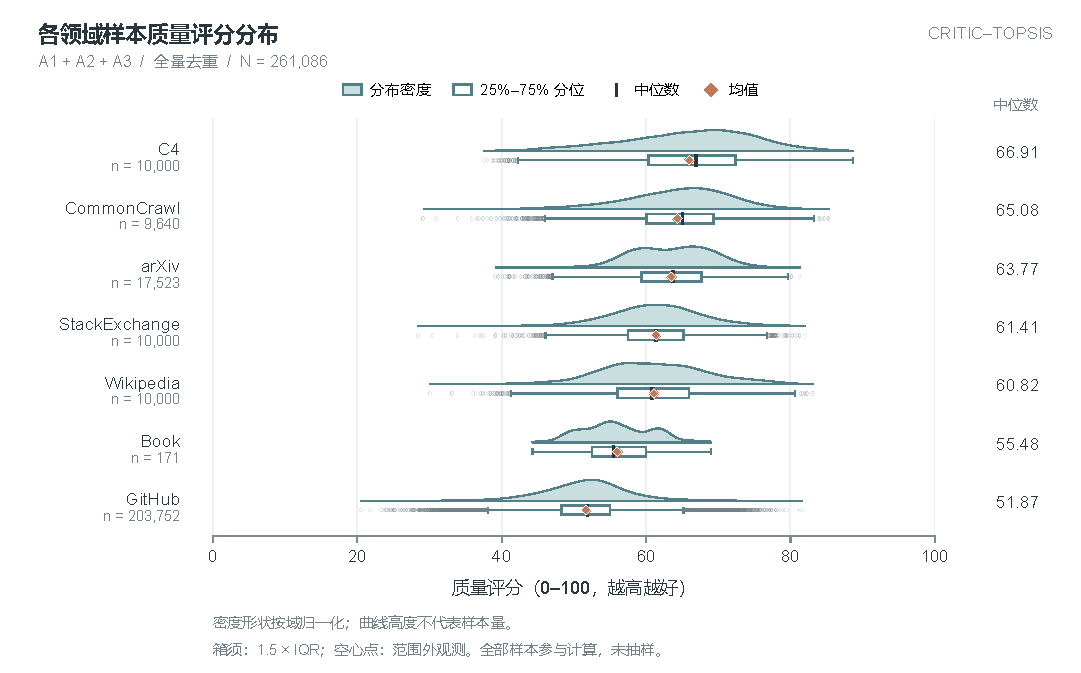
\includegraphics[width=\linewidth]{figures/q1-critic-topsis/nature-v1/figure01_domain_distribution_nature.pdf}
  \caption{各领域样本质量评分分布。完整数据口径和解释边界见配套图注。}
  \label{fig:q1-nature-01}
\end{figure}

\begin{figure}[htbp]
  \centering
  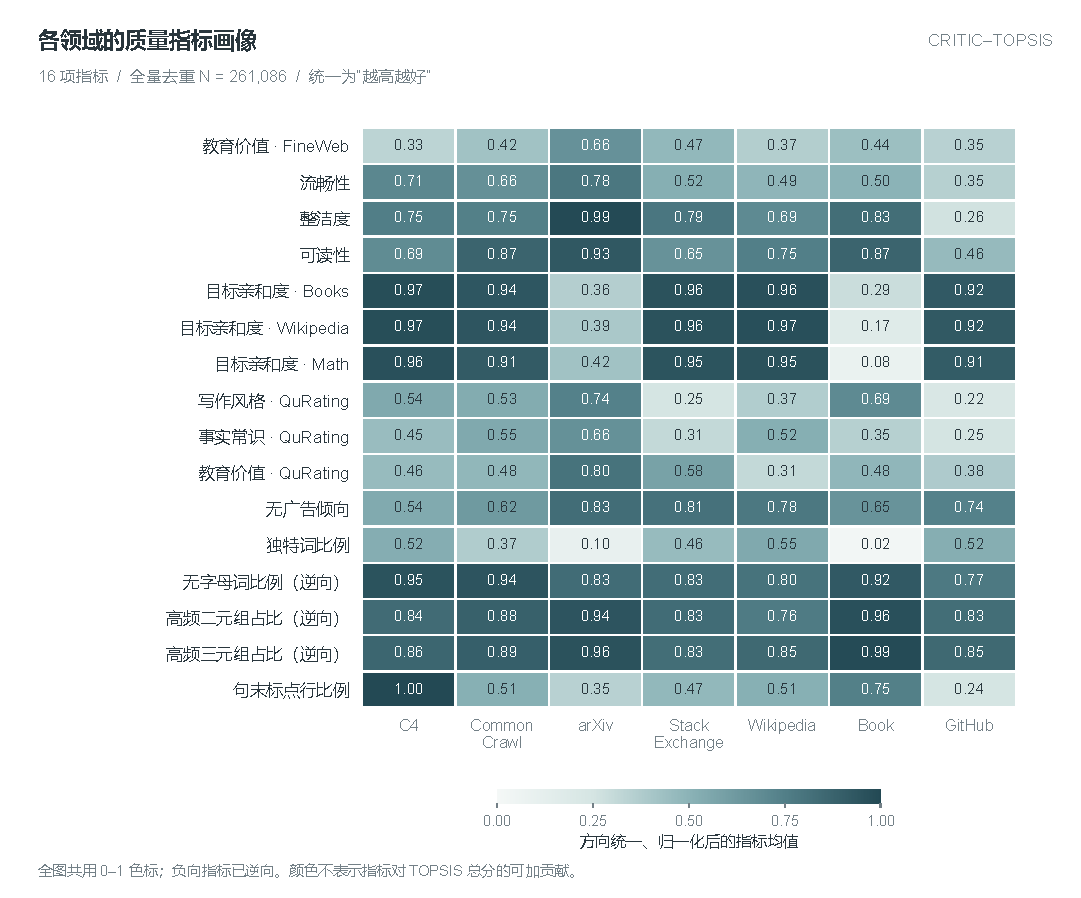
\includegraphics[width=\linewidth]{figures/q1-critic-topsis/nature-v1/figure02_indicator_heatmap_nature.pdf}
  \caption{各领域质量指标画像。完整数据口径和解释边界见配套图注。}
  \label{fig:q1-nature-02}
\end{figure}

\begin{figure}[htbp]
  \centering
  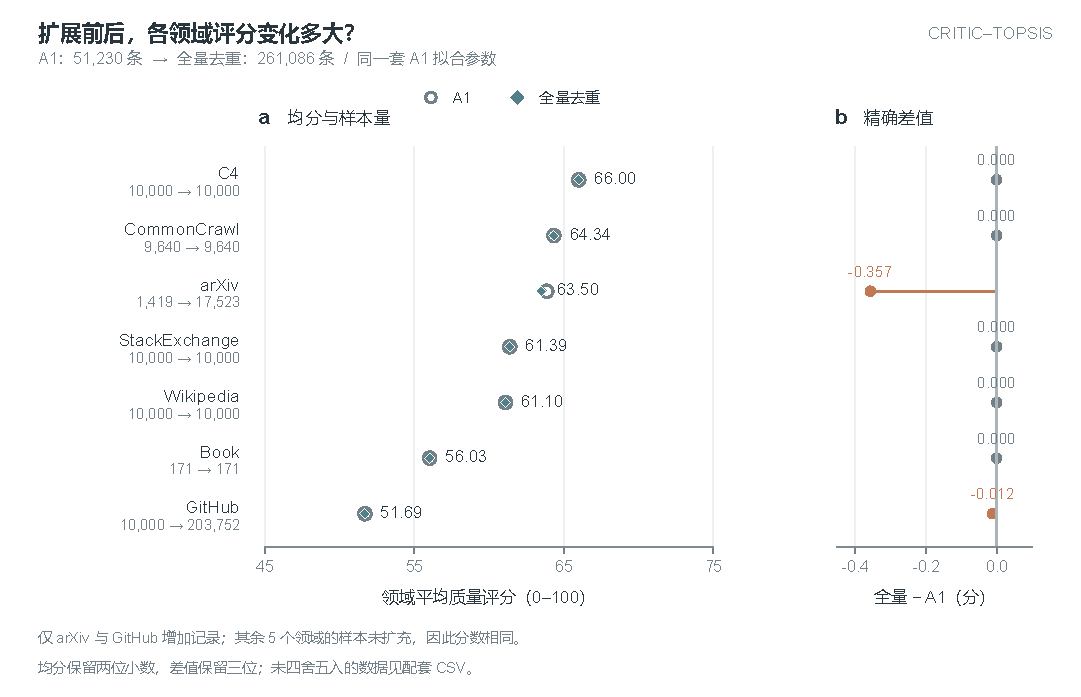
\includegraphics[width=\linewidth]{figures/q1-critic-topsis/nature-v1/figure03_A1_full_comparison_nature.pdf}
  \caption{A1 与全量领域评分对照（重绘）。完整数据口径和解释边界见配套图注。}
  \label{fig:q1-nature-03}
\end{figure}

\begin{figure}[htbp]
  \centering
  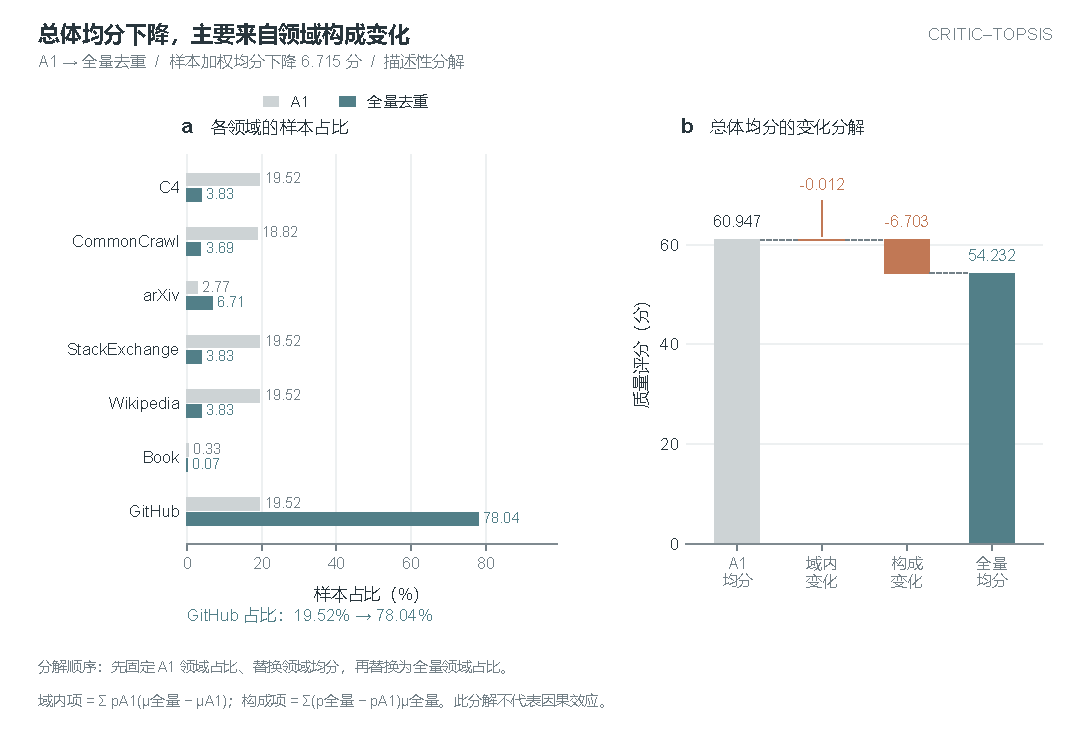
\includegraphics[width=\linewidth]{figures/q1-critic-topsis/nature-v1/figure04_composition_decomposition_nature.pdf}
  \caption{领域构成与总体均分分解。完整数据口径和解释边界见配套图注。}
  \label{fig:q1-nature-04}
\end{figure}

\begin{figure}[htbp]
  \centering
  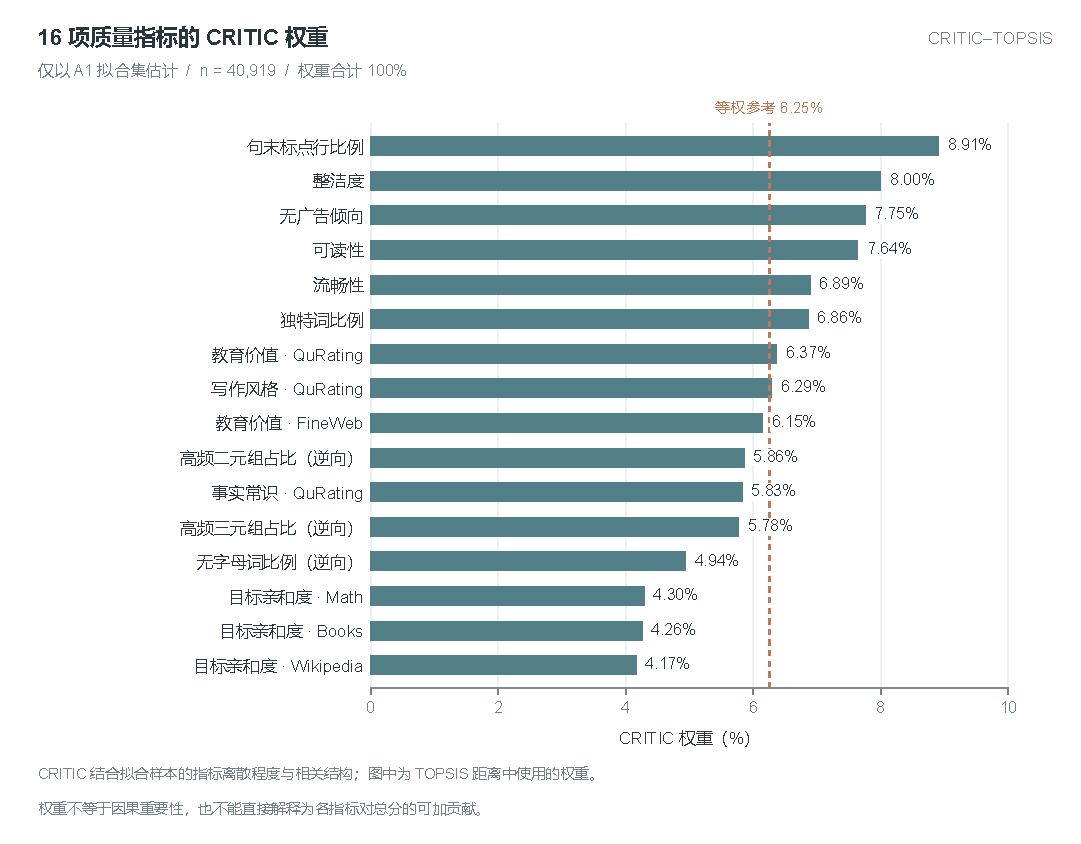
\includegraphics[width=\linewidth]{figures/q1-critic-topsis/nature-v1/figure05_critic_weights_nature.pdf}
  \caption{CRITIC 指标权重。完整数据口径和解释边界见配套图注。}
  \label{fig:q1-nature-05}
\end{figure}

\begin{figure}[htbp]
  \centering
  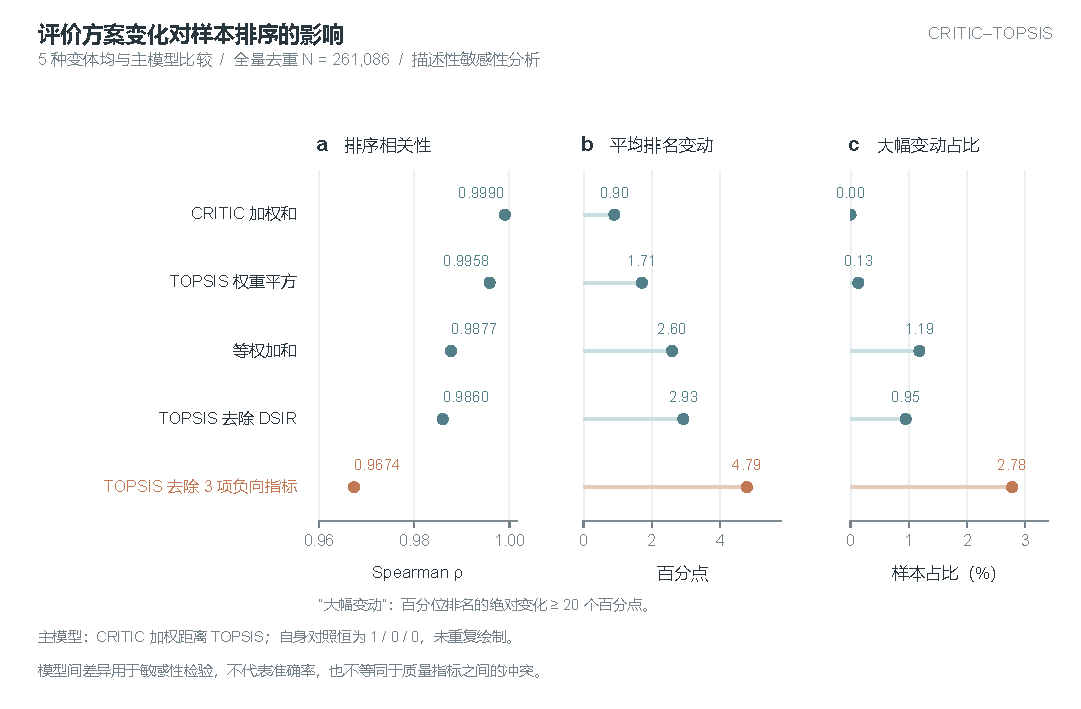
\includegraphics[width=\linewidth]{figures/q1-critic-topsis/nature-v1/figure06_model_sensitivity_nature.pdf}
  \caption{评价方案排序敏感性。完整数据口径和解释边界见配套图注。}
  \label{fig:q1-nature-06}
\end{figure}
